\chapter{Introduzione a RISC-V}

\begin{remark}
Negli anni Ottanta, John Hennessy e David Patterson svilupparono il processore MIPS, basato sull'idea di un \textit{Instruction Set} ridotto (RISC). L'obiettivo era semplificare le istruzioni per evitare stalli nell'elaborazione. Questa architettura rispecchiava una linea di produzione con diversi "stadi" (pipeline) in cui ogni operazione richiedeva lo stesso tempo delle altre. 
RISC-V nasce come naturale evoluzione open-source di questi concetti.
\end{remark}

\section{Storia e Caratteristiche Generali}

RISC-V è un'architettura ISA (\textit{Instruction Set Architecture}) basata su standard aperto e licenza libera. 
Proposta originariamente nel maggio 2010 dal Parallel Computing Laboratory (Par Lab) dell'Università di Berkeley (guidato dal Prof. David Patterson), si caratterizza per il nome "V" che ha molteplici significati:
\begin{itemize}
    \item È la \textbf{quinta versione} dell'ISA sviluppata a Berkeley.
    \item Il numero romano V rappresenta i \textbf{cinque stadi} della pipeline classica.
    \item Sta per \textbf{Variations} e \textbf{Vectors}, indicando la possibilità di aggiungere estensioni vettoriali.
\end{itemize}

Nel 2015 è nata la \textit{RISC-V Foundation} (oggi legata anche alla \textit{Linux Foundation}), che conta ormai centinaia di aziende e istituzioni membri.

\begin{remark}
Il nostro gruppo di ricerca al Politecnico lavora attivamente su implementazioni RISC-V sviluppate dall'ETH di Zurigo. Abbiamo anche esteso il processore con un acceleratore crittografico, motivo per cui nel corso vedremo alcune istruzioni orientate alla sicurezza. 
Inoltre, utilizzeremo un simulatore architetturale sviluppato internamente che ci permette di analizzare nel dettaglio cosa accade a livello micro-architetturale (dipendenze, stalli, ritardi), a differenza dei semplici emulatori disponibili online.
\end{remark}

\subsection{L'Architettura Load-Store}
RISC-V implementa una pura architettura \textbf{Load-Store}. 

\begin{definition}[Architettura Load-Store]
In un'architettura Load-Store, la memoria principale viene acceduta esclusivamente tramite istruzioni specifiche di caricamento (\texttt{load}) e salvataggio (\texttt{store}). Non è possibile eseguire un'operazione aritmetica o logica includendo un operando che risiede direttamente in memoria. I dati devono prima essere caricati nei registri interni del processore.
\end{definition}

\subsection{Tipi di Dati e Formato delle Istruzioni}
Nel nostro corso ci concentreremo sulla versione base a 32 bit, denominata \textbf{RV32I} (o \textbf{RV32G} quando include estensioni standard).
I tipi di dati supportati nativamente includono:
\begin{itemize}
    \item \textbf{Byte:} 8 bit.
    \item \textbf{Half Word:} 16 bit.
    \item \textbf{Word:} 32 bit.
    \item \textbf{Double Word:} 64 bit (non usata nella nostra versione a 32 bit).
    \item Numeri \textit{floating-point} a singola (32 bit) e doppia (64 bit) precisione.
\end{itemize}

La lunghezza delle istruzioni nel set base è \textbf{fissa a 32 bit}, il che semplifica notevolmente la fase di decodifica. 
Tuttavia, RISC-V permette un \textit{variable encoding} in blocchi multipli di 16 bit per ridurre la dimensione del codice (estensione C - Compressed). 

% FIGURA DA INSERIRE QUI
% Fonte: Slide 9
% Descrizione: Testo che mostra la codifica dei bit finali (11 per istruzioni a 32 bit).
\begin{figure}[H]
    \centering
    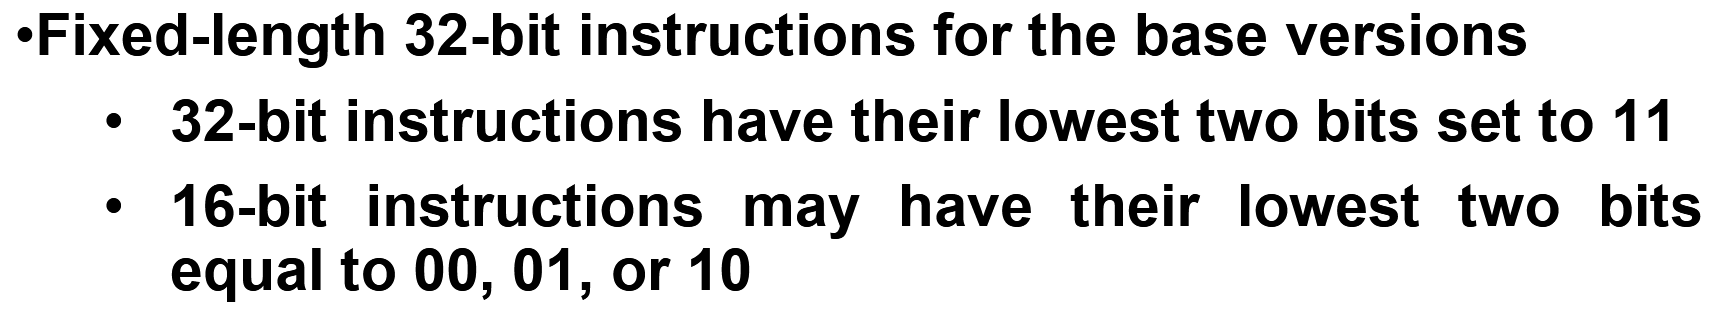
\includegraphics[width=0.7\textwidth]{capitoli/03_RISC-V_Introduction/images/riscv_length.png}
    \caption{I 2 bit meno significativi indicano la lunghezza dell'istruzione: \texttt{11} identifica istruzioni a 32 bit.}
    \label{fig:riscv_length}
\end{figure}

Il sistema di memoria utilizzato è \textbf{Little-Endian}: l'indirizzo base di una Word o Half-Word punta al suo byte meno significativo. Le istruzioni a 32 bit devono essere rigorosamente \textbf{allineate in memoria} (indirizzi multipli di 4).

\section{Rappresentazione dei Dati}

\subsection{Interi e Complemento a Due}
L'intera aritmetica del processore per i numeri interi si basa sul \textbf{complemento a due (2C)}. Questo è fondamentale per gestire correttamente somme, sottrazioni e salti condizionati.
Dato un numero binario \( A \) di \( N \) bit, il complemento a due è definito come:
\[ -A = 2^N - A = \overline{A} + 1 \]

\begin{example}
Lavorando su 3 bit, l'intervallo di rappresentazione va da \(-4\) a \(+3\). 
Il valore binario \texttt{100} rappresenta \(-4_{10}\) se valutato in complemento a due, ma rappresenta \(+4_{10}\) se considerato \textit{unsigned}. Le istruzioni assembler dovranno perciò differenziare le operazioni con segno da quelle senza segno (es. \texttt{slt} vs \texttt{sltu}).
\end{example}

\begin{figure}[H]
    \centering
    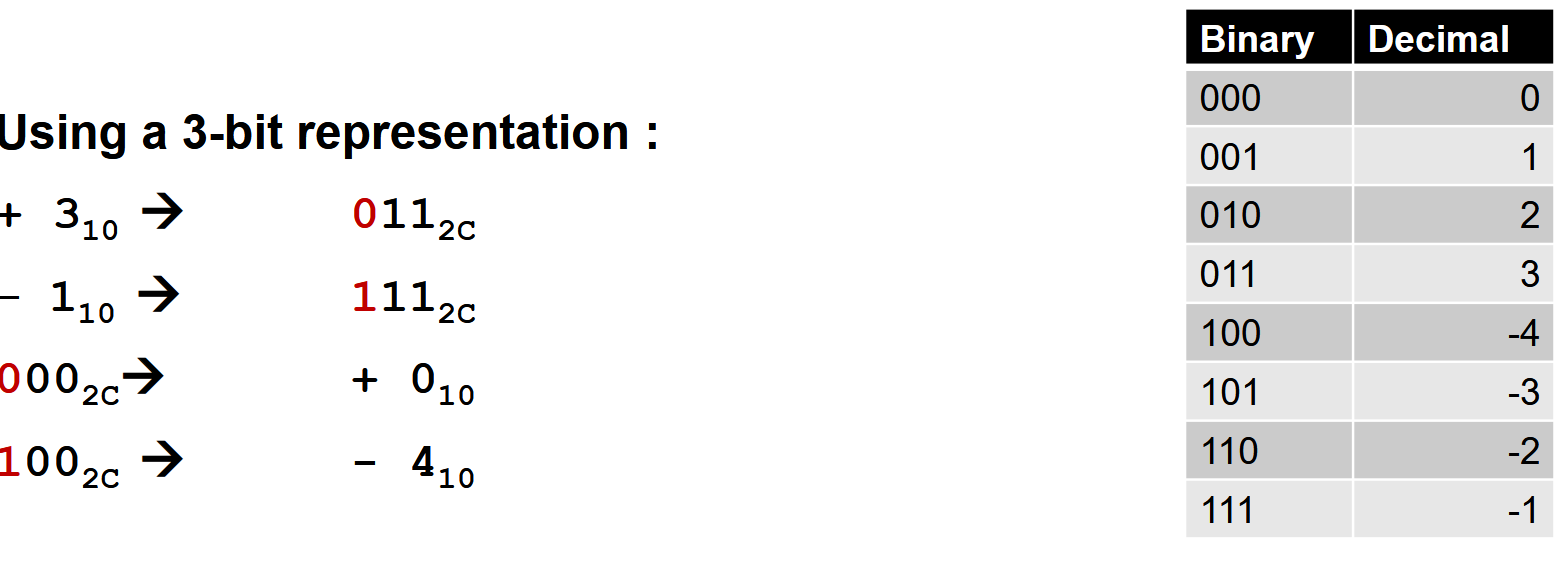
\includegraphics[width=0.8\textwidth]{capitoli/03_RISC-V_Introduction/images/complemento_due.png}
    \caption{Esempio di rappresentazione in complemento a due su 3 bit.}
    \label{fig:complemento_due}
\end{figure}

\subsection{Floating-Point (IEEE 754)}
Se si adotta l'estensione F o D, RISC-V utilizza lo standard IEEE 754. Per i 32 bit, la word è divisa in:
\begin{itemize}
    \item \textbf{Segno:} 1 bit
    \item \textbf{Esponente:} 8 bit
    \item \textbf{Mantissa:} 23 bit
\end{itemize}

% FIGURA DA INSERIRE QUI
% Fonte: Slide 8
% Descrizione: Schema dei bit della rappresentazione IEEE 754 e un esempio di calcolo.
\begin{figure}[H]
    \centering
    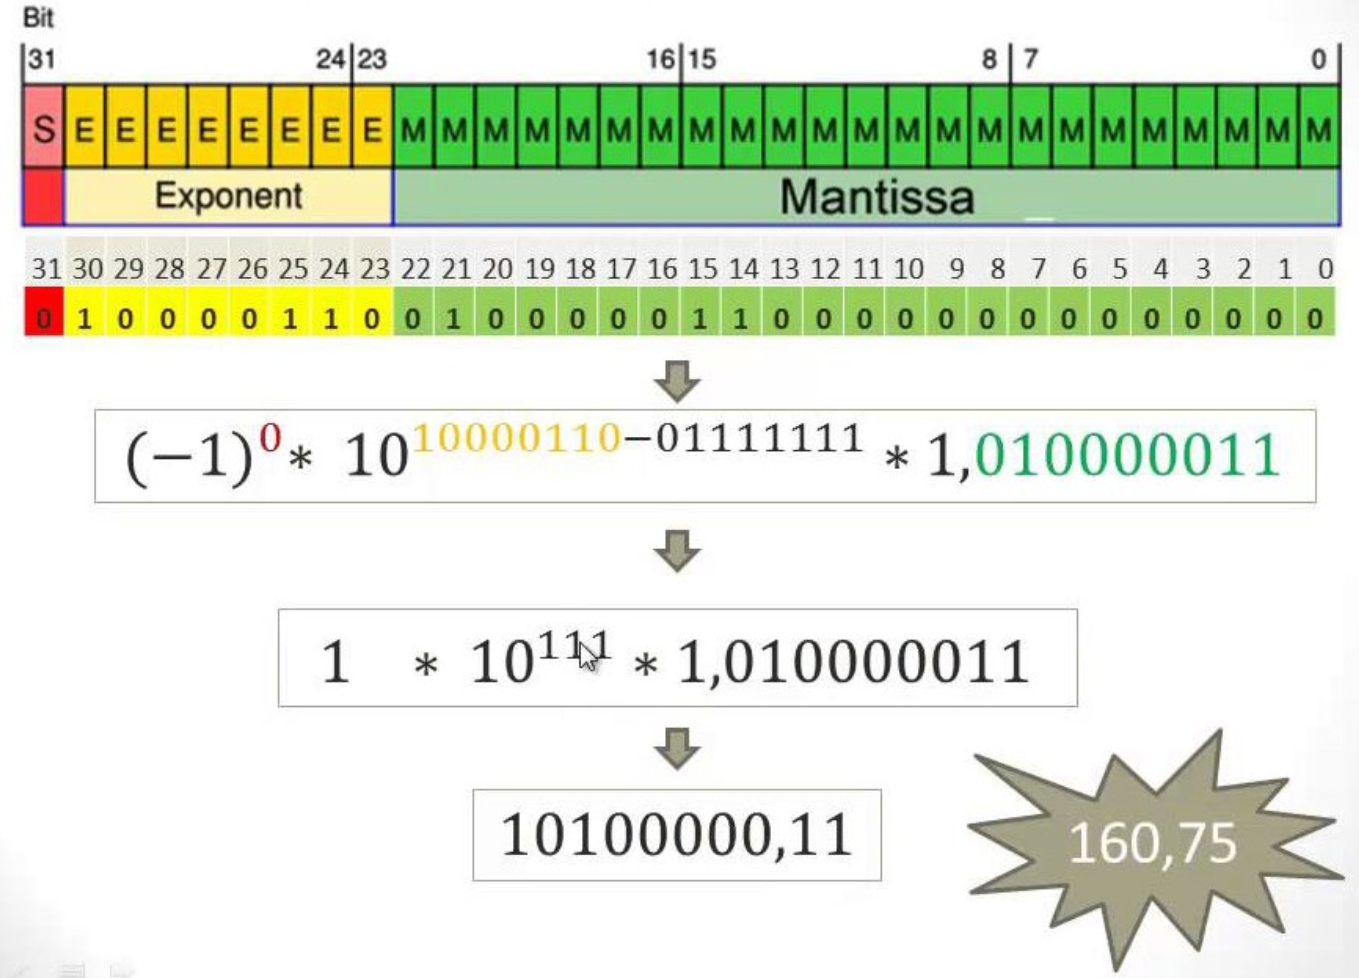
\includegraphics[width=0.5\textwidth]{capitoli/03_RISC-V_Introduction/images/ieee754_format.png}
    \caption{Formato a 32 bit IEEE 754 per i numeri in virgola mobile.}
    \label{fig:ieee754}
\end{figure}

\section{Organizzazione dell'Instruction Set e Registri}

La modularità è il cuore di RISC-V. Un processore standard viene definito tramite sigle, ad esempio \textbf{RV64IMAFD} (spesso abbreviato in \textbf{RV64G}, \textit{General-purpose}):
\begin{itemize}
    \item \textbf{I:} Base integer ISA (32 registri interi).
    \item \textbf{M:} Moltiplicazione e divisione.
    \item \textbf{A:} Istruzioni atomiche.
    \item \textbf{F, D:} Floating-point a singola e doppia precisione.
\end{itemize}

% FIGURA DA INSERIRE QUI
% Fonte: Slide 10
% Descrizione: Tabella completa delle estensioni (I, E, M, A, F, D, Q, L, C, V, ecc.).
\begin{figure}[H]
    \centering
    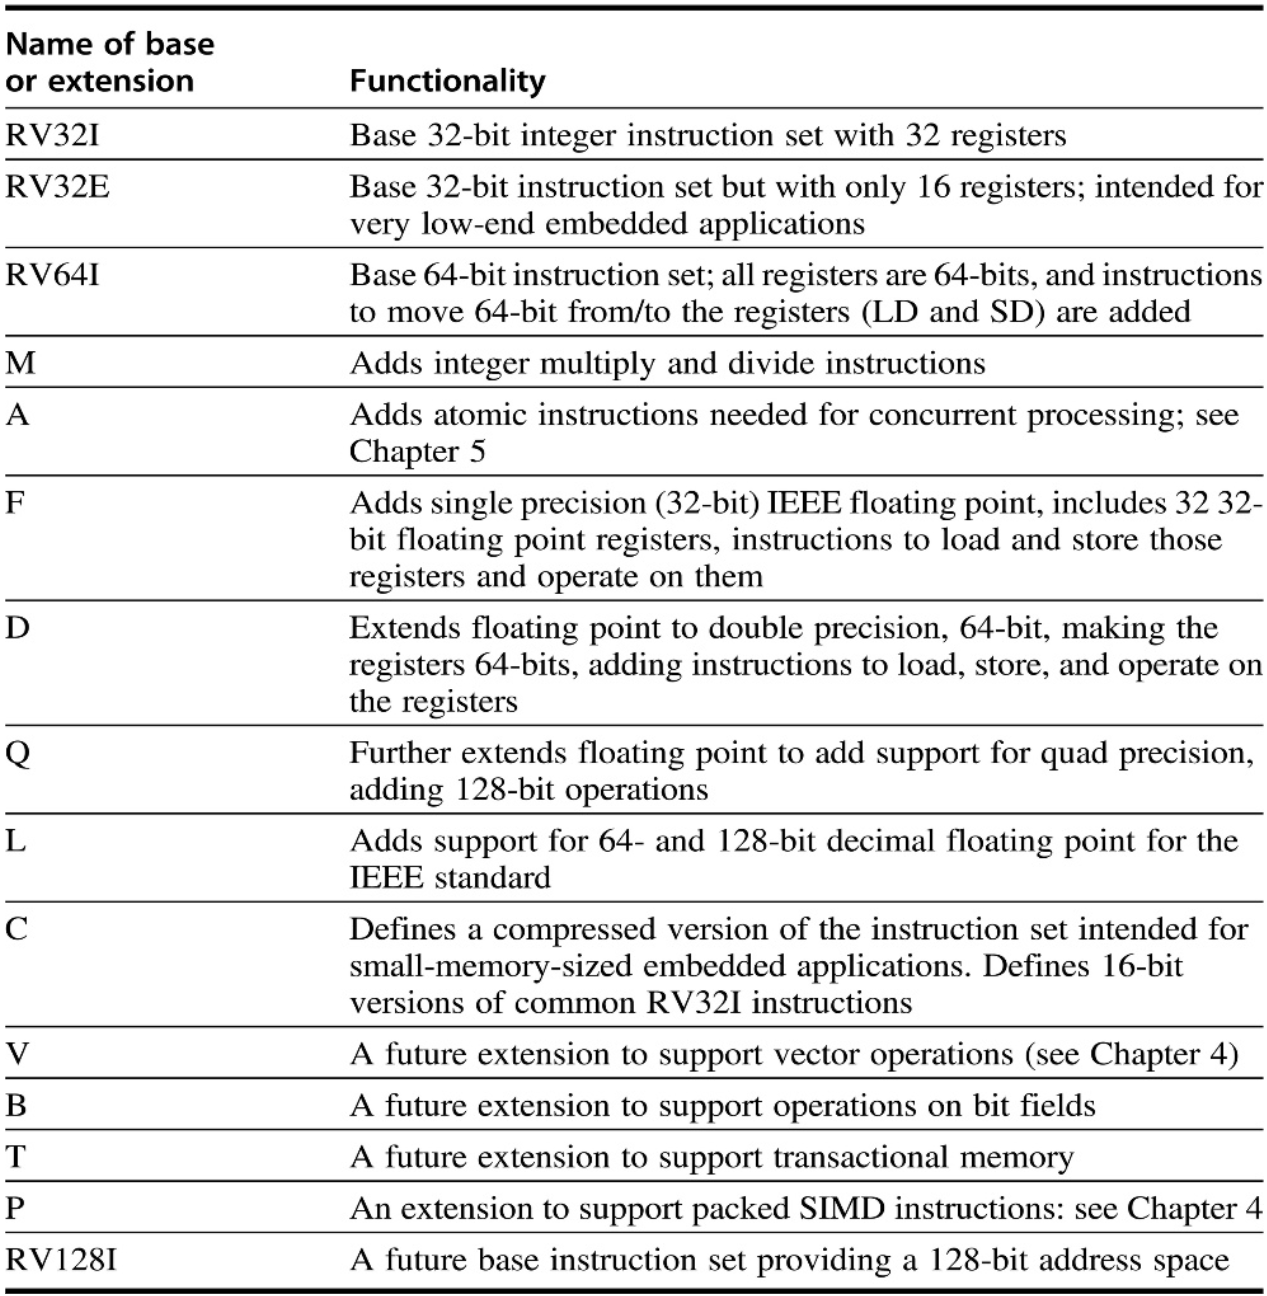
\includegraphics[width=0.7\textwidth]{capitoli/03_RISC-V_Introduction/images/riscv_extensions_table.png}
    \caption{Principali estensioni dell'Instruction Set RISC-V.}
    \label{fig:riscv_extensions}
\end{figure}

\subsection{I Registri}
La versione a 32 bit (RV32I) possiede \textbf{32 registri generici interi} da 32 bit, numerati da \texttt{x0} a \texttt{x31}, più il Program Counter (\texttt{PC}).
\begin{itemize}
    \item \textbf{Il registro \texttt{x0} (zero):} È hardwired a 0. Non può essere modificato e restituisce sempre 0. È estremamente utile per sintetizzare altre operazioni (es. copiare registri o forzare zeri).
    \item \textbf{Registri Floating Point:} Se l'estensione è attiva, si aggiungono 32 registri \texttt{f0} - \texttt{f31}.
\end{itemize}

\begin{remark}
Lo standard ABI (\textit{Application Binary Interface}) definisce nomi specifici per i registri in base al loro ruolo nelle funzioni C/C++ (es. \texttt{ra} per \texttt{x1} come Return Address, \texttt{sp} per \texttt{x2} come Stack Pointer, \texttt{a0-a7} per gli argomenti). 
Tuttavia, in questa fase introduttiva in Assembly puro, \textbf{utilizzeremo la notazione nativa} (\texttt{x0, x1, \dots}) e non ci preoccuperemo delle convenzioni di chiamata delle funzioni.
\end{remark}

% FIGURA DA INSERIRE QUI
% Fonte: Slide 12
% Descrizione: Tabella dei registri RV32I con nomi ABI e descrizioni (x0=zero, x1=ra, ecc.).
\begin{figure}[H]
    \centering
    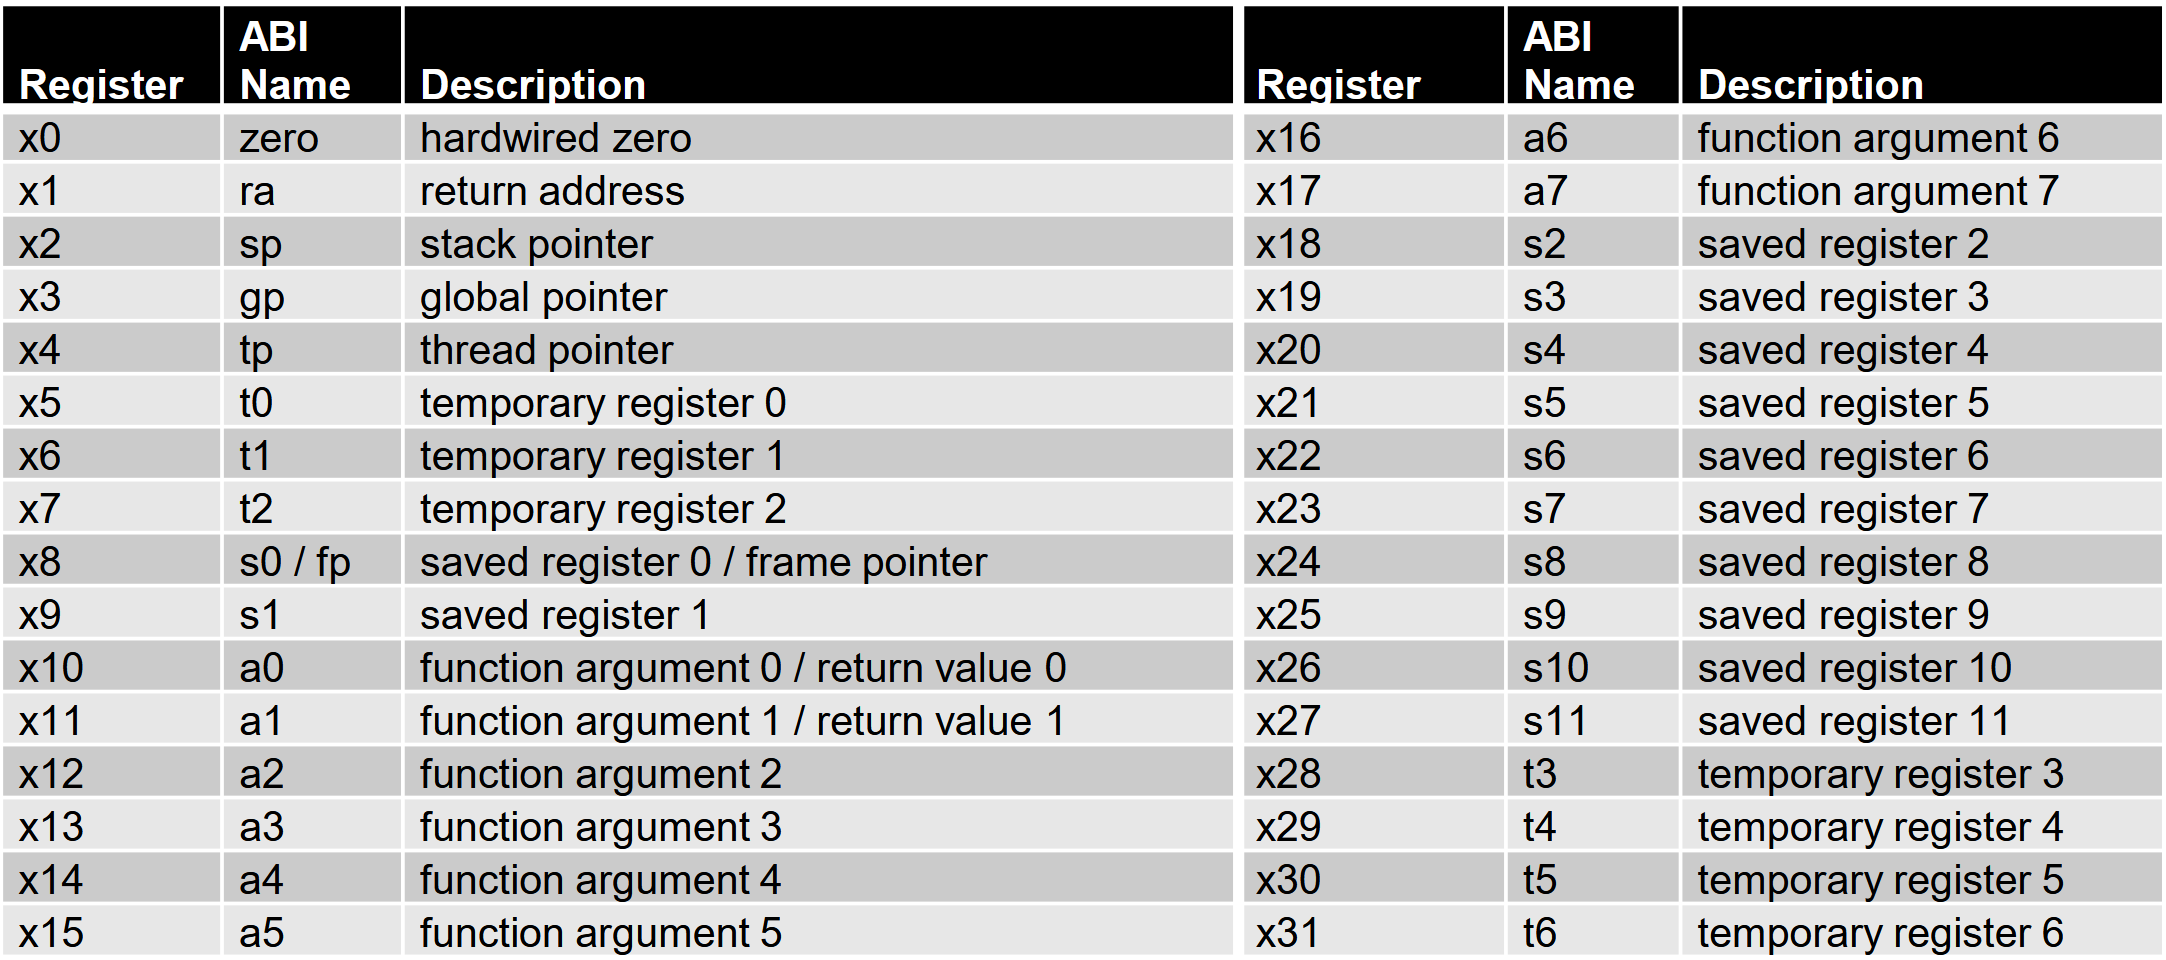
\includegraphics[width=0.9\textwidth]{capitoli/03_RISC-V_Introduction/images/riscv_registers_abi.png}
    \caption{Banco registri RV32I con le relative convenzioni ABI.}
    \label{fig:riscv_registers}
\end{figure}

\section{Modi di Indirizzamento}
L'architettura supporta tre modi principali per l'indirizzamento di dati in memoria e istruzioni:

\begin{enumerate}
    \item \textbf{Immediate (Immediato):} Il dato è contenuto direttamente nell'istruzione (tipicamente 12 bit con estensione del segno).
    \[ \texttt{addi x1, x2, 32} \quad \Rightarrow \quad x1 \leftarrow x2 + 32 \]
    \[ \texttt{addi x1, x0, 32} \quad \Rightarrow \quad x1 \leftarrow 32 \]
    
    \item \textbf{Displacement (Spiazzamento):} Utilizza una base salvata in un registro più un offset (12 bit) costante.
    \[ \texttt{lw x1, 30(x2)} \quad \Rightarrow \quad x1 \leftarrow \text{MEM}[x2 + 30] \]
    
    \item \textbf{Register Indirect (Indiretto a registro):} Non esiste come modalità nativa, ma è un caso particolare del Displacement con offset nullo.
    \[ \texttt{lw x1, 0(x2)} \quad \Rightarrow \quad x1 \leftarrow \text{MEM}[x2] \]
\end{enumerate}

Tramite l'uso di \texttt{x0}, si può simulare anche un \textbf{indirizzamento assoluto} in un intervallo ristretto (i primi 4 KB di memoria), scrivendo \texttt{lw x1, 30(x0)}.

\section{Formato delle Istruzioni}
Le istruzioni a 32 bit sono suddivise in categorie di codifica. Tutte mantengono l'\texttt{Opcode} nei 7 bit meno significativi. I formati principali sono:

\begin{itemize}
    \item \textbf{R-Type (Register):} Operazioni tra registri (es. somma). Struttura: \texttt{Opcode(7)}, \texttt{rd(5)}, \texttt{func3(3)}, \texttt{rs1(5)}, \texttt{rs2(5)}, \texttt{func7(7)}.
    \item \textbf{I-Type (Immediate):} Operazioni con immediati o Load. L'immediato a 12 bit sostituisce \texttt{rs2} e \texttt{func7}.
    \item \textbf{S-Type (Store):} Utilizzato per salvare in memoria. Il campo immediato a 12 bit è "spezzato" (\texttt{Imm[11:5]} e \texttt{Imm[4:0]}) per mantenere il registro sorgente \texttt{rs2} nella stessa posizione delle R-Type, semplificando l'hardware decodificatore.
    \item \textbf{U-Type (Upper Immediate):} Istruzioni con immediati estesi a 20 bit (es. \texttt{LUI}, \texttt{AUIPC}), usate per gestire grandi costanti e indirizzamenti a lungo raggio.
\end{itemize}

% FIGURA DA INSERIRE QUI
% Fonte: Slide 18-21 (Creare o usare una vista combinata)
% Descrizione: Tabelle o schemi a blocchi dei formati R, I, S, U.
\begin{figure}[H]
    \centering
    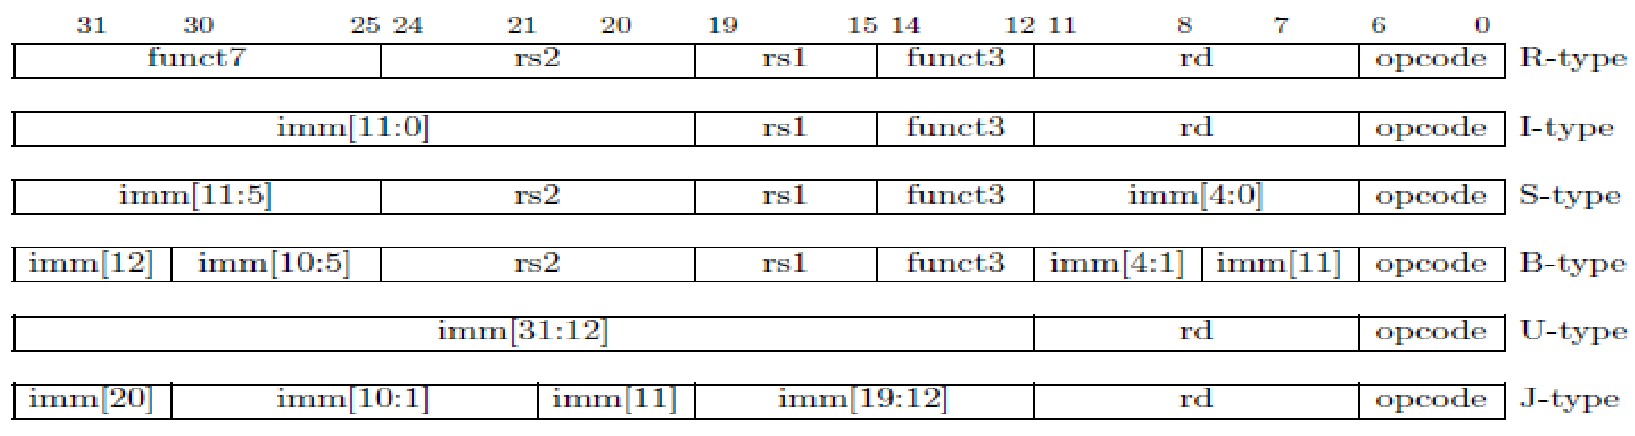
\includegraphics[width=0.9\textwidth]{capitoli/03_RISC-V_Introduction/images/riscv_formats.png}
    \caption{Struttura dei formati R, I, S, U dell'instruction set RISC-V.}
    \label{fig:riscv_formats}
\end{figure}

\section{Analisi delle Istruzioni Base}

\subsection{Load e Store}
Gestiscono il trasferimento dati memoria-registri. Nella sintassi, la Load ha il registro di destinazione come primo operando, mentre la Store ha il registro sorgente come primo operando.

\begin{itemize}
    \item \texttt{lw x1, 28(x8)}: Carica una word (32 bit).
    \item \texttt{lb x1, 28(x8)}: Carica un byte con \textbf{estensione del segno}.
    \item \texttt{lbu x1, 28(x8)}: Carica un byte (\textit{unsigned}) con estensione di zeri.
    \item \texttt{sw x2, 28(x8)}: Salva una word.
    \item \texttt{sb x2, 28(x8)}: Salva un solo byte.
\end{itemize}

\begin{remark}[L'importanza dell'estensione del segno]
Quando carichiamo un byte (8 bit) in un registro a 32 bit (\texttt{lb}), dobbiamo replicare il bit più significativo (il segno) nei restanti 24 bit a sinistra. Questo serve a preservare il valore matematico del numero in complemento a due (es. \(-3\) su 8 bit deve rimanere \(-3\) su 32 bit). Se usiamo \texttt{lbu}, i 24 bit aggiuntivi vengono forzati a zero.
\end{remark}

\subsubsection{Caricamento di indirizzi e pseudo-istruzione LA}
Poiché l'immediato del displacement è limitato a 12 bit (da -2048 a +2047), indirizzare variabili arbitrarie in memoria richiede un trucco. Il compilatore offre la pseudo-istruzione \texttt{la} (\textit{Load Address}):

\[ \texttt{la x5, var} \]

In realtà, questa viene tradotta in due istruzioni reali che sfruttano il PC e un immediato superiore:
\begin{enumerate}
    \item \texttt{auipc x5, <upper\_20\_bits>}: Aggiunge i 20 bit alti (shiftati a sinistra) al Program Counter e salva in \texttt{x5}.
    \item \texttt{addi x5, x5, <lower\_12\_bits>}: Aggiusta i 12 bit inferiori per centrare l'indirizzo esatto.
\end{enumerate}

\subsection{Operazioni Aritmetico-Logiche (ALU)}
L'ALU esegue istruzioni su registri o tra registri e immediati (es. \texttt{add}, \texttt{addi}, \texttt{sub}, \texttt{and}, \texttt{sll}).
Il registro \texttt{x0} è vitale per sintetizzare istruzioni "mancanti" nel set:

\begin{example}
\textbf{Caricare una costante in un registro:}
\[ \texttt{addi x1, x0, 10} \quad (\text{Esegue } x1 \leftarrow 0 + 10) \]

\textbf{Copiare il contenuto di un registro (Move):}
\[ \texttt{add x1, x0, x2} \quad (\text{Esegue } x1 \leftarrow 0 + x2) \]

\textbf{No-Operation (NOP):}
\[ \texttt{addi x0, x0, 0} \quad (\text{Aggiunge 0 a 0 e salva nel cestino } x0) \]
\end{example}

\subsection{Salti e Diramazioni (Branches e Jumps)}
RISC-V utilizza istruzioni di confronto e salto integrate (senza usare \textit{Condition Codes/Flags} separati come in altre ISA).

\subsubsection{Salti Incondizionati}
Le istruzioni \texttt{jal} (\textit{Jump And Link}) e \texttt{jalr} saltano a un indirizzo e salvano l'indirizzo di ritorno nel registro di destinazione.
\begin{itemize}
    \item \textbf{Jump semplice:} \texttt{j label} viene tradotto come \texttt{jal x0, label} (salta e scarta il ritorno in \texttt{x0}).
    \item \textbf{Chiamata a funzione:} \texttt{call label} salva il ritorno di default in \texttt{x1} (\texttt{ra}).
    \item \textbf{Ritorno:} \texttt{ret} viene tradotto come \texttt{jalr x0, 0(x1)} (salta all'indirizzo in \texttt{x1}).
\end{itemize}

\subsubsection{Salti Condizionati (Branches)}
Le istruzioni confrontano direttamente due registri (es. \texttt{beq}, \texttt{bne}, \texttt{blt}, \texttt{bge}). L'immediato per il target del salto è a 12 bit, limitando il raggio del salto a \(\pm 4\) KB dal PC attuale.
Anche qui, l'uso di \texttt{x0} permette pseudo-istruzioni eleganti:
\begin{itemize}
    \item \texttt{beqz x3, label} $\rightarrow$ Tradotta come \texttt{beq x3, x0, label} (Salta a label se il registro x3 è uguale a zero.)
    \item \texttt{bgtz x3, label} $\rightarrow$ Tradotta come \texttt{blt x0, x3, label} (salta se \(0 < x3\)).
\end{itemize}

\begin{remark}[Testare lo Zero in modo asimmetrico]
Per generare un valore booleano basato su una condizione, possiamo usare \texttt{slt} (\textit{Set Less Than}). 
Ad esempio, se vogliamo settare \texttt{x1 = 1} se \texttt{x2 == 0}, non esiste un'istruzione nativa \texttt{seqz}. Il compilatore utilizzerà:
\[ \texttt{sltiu x1, x2, 1} \]
Ovvero: Setta \texttt{x1} a 1 se \texttt{x2} è strettamente minore di 1 valutato senza segno (l'unico intero \textit{unsigned} minore di 1 è lo 0).
\end{remark}